\documentclass[conference]{IEEEtran}
\IEEEoverridecommandlockouts
\usepackage{amsmath,amssymb}
\usepackage{graphicx}
\usepackage{booktabs}
\usepackage{array}
\usepackage{xcolor}
\usepackage{tikz}
\usetikzlibrary{positioning,arrows.meta,fit,backgrounds}
\usepackage{url}
\usepackage[hidelinks]{hyperref}

\newcommand{\tool}{\texttt{dc-profile}}
\begin{document}

\title{AI Demand Controller for Resource-Aware Diagnostic Evidence Delivery in Codebase Tuning}

\author{\IEEEauthorblockN{Gowtham Balasubramanian}
\IEEEauthorblockA{Email: gowthamkopite@gmail.com}}

\maketitle

\begin{abstract}
Coding agents asked to make a repository faster need to know where time is
spent, but profiler output is costly to collect and can be far longer than an
agent can usefully read. A \emph{demand controller} sits between the agent and
the profiler: it admits requests against a fixed allowance, shows the remaining
allowance, and returns a compressed artifact instead of the raw profile.
Profiler-guided agents, cost-aware profiling harnesses and budget-aware tool
use already exist. Our contribution is a controlled comparison that holds the
agent, model, prompt, allowance and profile data fixed and varies only the
evidence \emph{format} (none, truncated cProfile dump, ranked hotspot table)
and, across two pre-registered pilots, the \emph{delivery mode} (on demand or
automatic). Each pilot uses 18 SWE-fficiency tasks from 8 repositories, one
agent, and one run per task and condition. Offered on demand (Pilot~1), the
tool was called in 8 of 64 runs, and no run in the pre-registered set
received a profile.
Delivered automatically (Pilot~2), the profile reached all 34 valid tool runs,
but no agent asked for a second one. Harmonic-mean speedup ratios were 0.55
with no tool, 0.56 with the dump and 0.81 with the ranked table. Every paired
95\% interval includes zero, and the ranked table's lead comes from two
tasks. Profile delivery displaced self-profiling in the shell (6 of 18 runs
without the tool, 0 and 1 with it). From the observed variance, a confirmatory
study needs about 145 tasks to detect a 10\% difference between formats. The
pre-registration, code, prompts, logs and analysis scripts are released.
\end{abstract}

\begin{IEEEkeywords}
LLM agents, performance profiling, budget-aware tooling, code optimization,
tool output compression, pre-registration
\end{IEEEkeywords}

\section{Introduction}

Large language model (LLM) agents can read a repository, edit it, and run its
tests inside a container~\cite{yang2024sweagent,xia2024agentless}, and
benchmarks such as SWE-bench measure whether they resolve real
issues~\cite{jimenez2024swebench,hou2024llm4se}. Performance work is harder:
the agent must keep behaviour unchanged while making a workload faster, and
where time goes is often not obvious from the code. Benchmarks built from real
performance-improving commits, namely SWE-fficiency~\cite{ma2025swefficiency},
GSO~\cite{shetty2025gso} and SWE-Perf~\cite{he2025sweperf}, report that agents
reach a small fraction of expert speedups and list poor bottleneck
localization among the main failure modes.

A profiler is the standard localization tool, but giving one to an agent is
not free. Profiling costs wall-clock time; a full profile can list thousands
of functions, and models use the middle of long contexts less
reliably~\cite{liu2024lost}; and profiles can mislead, because profilers
misattribute time~\cite{mytkowicz2010evaluating} and the hottest function is
not always the one whose optimization shortens end-to-end
runtime~\cite{curtsinger2015coz}. We call the layer that manages this
trade-off a \emph{demand controller}: it admits a profiling request against a
visible allowance and returns a compressed artifact rather than the raw
profile.

\textbf{What is and is not new.} Each ingredient has precedent.
PerfAgent~\cite{deng2026perfagent} feeds curated sampling-profiler summaries to
an agent inside a loop that re-profiles and re-tests every patch;
ProfileWeaver~\cite{ding2026profileweaver} selects profiling actions by
expected insight per cost under token, time and iteration budgets;
BATS~\cite{liu2025bats} shows a remaining-budget tracker to a tool-using
agent; and continuous profilers such as GWP~\cite{ren2010gwp} have long bounded
profiling overhead by sampling. Our controller is a deliberately simple
combination of these ideas and is not claimed as a contribution in itself.
What prior systems do not isolate is the effect of the evidence
\emph{format}: they bundle the profiler with loop control, verification and
selective testing, and none reports whether a ranked summary beats a plain
truncated dump when everything else is held fixed (Table~\ref{tab:position}).
The contributions of this paper are therefore methodological and empirical:
\begin{itemize}
\item A controlled design that varies only the rendering of identical profile
  data (none, dump, ranked table), with the allowance meter kept on the host
  where the agent cannot alter it (Section~\ref{sec:design}).
\item Two pre-registered pilots on SWE-fficiency that also vary the delivery
  mode. Agents almost never request on-demand evidence, whereas automatic
  delivery reaches every run and replaces self-profiling
  (Section~\ref{sec:results}).
\item A complete, reproducible protocol: software versions, seeds, resource
  limits, a baseline-relative correctness rule for local reproduction,
  per-task results, a run-by-run audit, and a power analysis that sizes a
  confirmatory study (Sections~\ref{sec:method} and~\ref{sec:discussion}).
\end{itemize}
We do not claim that any format improves optimization. Both pilots are too
small for that, and we report them as pilots.

\section{Related Work}

\textbf{Benchmarks.} SWE-fficiency~\cite{ma2025swefficiency} has 498 tasks
from nine Python repositories. Each gives a repository and a slow workload and
scores a patch by the \emph{speedup ratio} (SR), the agent's speedup divided by
the expert's, aggregated by a harmonic mean; patches failing the selected
tests count as incorrect. GSO~\cite{shetty2025gso} and
SWE-Perf~\cite{he2025sweperf} are built similarly from commit histories, and
PIE~\cite{shypula2023pie} studies performance edits to single programs. We use
SWE-fficiency because its harness, workloads and prompt are released.

\textbf{Execution feedback for optimization.}
EffiLearner~\cite{huang2024effilearner} feeds line-level time and memory
profiles of generated functions back to the model, and
PerfCodeGen~\cite{peng2025perfcodegen} feeds back the most expensive unit test.
Both work on single functions and fix the feedback format.
PerfAgent~\cite{deng2026perfagent}, the closest work, adds py-spy hotspot
summaries, a loop that rejects the first passing patch, and selective tests.
It also reports that an agent merely \emph{told} how to use the profiler did
much worse (16.7\% vs.\ 39.2\% hack-adjusted expert-matching patches on GSO),
which matches our delivery-mode finding. It does not compare formats.
ProfileWeaver~\cite{ding2026profileweaver}, a poster, normalizes several HPC
profilers into a shared summary under a cost-aware controller and reports no
controlled comparison.

\textbf{Resource-aware tool use.} BATS~\cite{liu2025bats} gives web-search
agents a budget tracker and budget-aware planning, and shows that a larger
tool-call budget alone does not raise accuracy. SMART~\cite{qian2025smart} and
OTC~\cite{wang2025otc} train models to avoid unnecessary tool calls. These
works ration \emph{how many} calls an agent makes. We hold the allowance fixed
and ask whether \emph{what a call returns} matters. Our meter is the
non-learned analogue of BATS's tracker, applied to a costly diagnostic tool.

\textbf{Profiling under a budget and output compression.} GWP~\cite{ren2010gwp}
keeps fleet-wide profiling overhead below 0.01\% by sampling machines and
events. Causal profiling~\cite{curtsinger2015coz} and flame
graphs~\cite{gregg2016flame} target human analysts. For agents,
Squeez~\cite{kovacs2026squeez} learns to prune tool output, and SWE-agent showed
that how command output is displayed changes success~\cite{yang2024sweagent}.
A ranked hotspot table is a hand-written, domain-specific compressor.

\begin{table}[t]
\caption{Positioning. ``Format isolated'': the work compares evidence
renderings with agent, budget and profile data held fixed.}
\label{tab:position}
\centering
\scriptsize
\setlength{\tabcolsep}{2pt}
\begin{tabular}{@{}>{\raggedright\arraybackslash}p{2.05cm}>{\raggedright\arraybackslash}p{1.95cm}>{\raggedright\arraybackslash}p{1.95cm}>{\centering\arraybackslash}p{0.75cm}>{\raggedright\arraybackslash}p{0.95cm}@{}}
\toprule
Work & Evidence & Budget control & Format isolated & Setting \\
\midrule
EffiLearner~\cite{huang2024effilearner} & line time/memory profile & fixed iterations & no & functions \\
PerfCodeGen~\cite{peng2025perfcodegen} & slowest test & fixed iterations & no & functions \\
PerfAgent~\cite{deng2026perfagent} & py-spy hotspots & \$ per task, attempts & no & repos \\
ProfileWeaver~\cite{ding2026profileweaver} & multi-profiler summary & token/time/iter.\ & no & HPC \\
BATS~\cite{liu2025bats} & (web search) & visible call budget & no & search \\
SMART~\cite{qian2025smart}, OTC~\cite{wang2025otc} & (generic tools) & learned & no & QA \\
This work & cProfile, 2 renderings & host-side meter, 4 calls & yes & repos \\
\bottomrule
\end{tabular}
\end{table}

\section{Demand Controller Design}
\label{sec:design}

\textbf{Model.} A tool $T$ maps a program $P$ and workload $W$ to an evidence
artifact $E=T(P,W)$; the agent reads $E$ and produces a patch $\Delta$, scored
by correctness and speedup. In general the controller holds a budget
$B=(A_{\max},T_{\max},K_{\max})$ on calls, profiling time and evidence tokens.
The pilots implement only $A_{\max}=4$ calls per task. Profiling time comes out
of the agent's wall-clock limit (except Pilot~2's automatic profile, which runs
before the clock starts in both tool conditions), and token cost is bounded by
the format.

\begin{figure}[t]
\centering
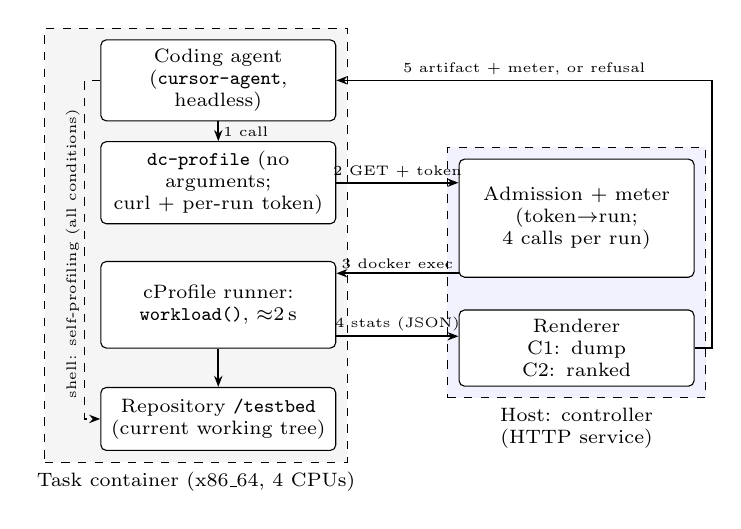
\begin{tikzpicture}[
  font=\scriptsize,
  box/.style={draw, rounded corners=2pt, align=center, text width=2.75cm,
              minimum height=0.8cm, fill=white},
  arr/.style={-{Stealth[length=4pt]}, semithick},
  lab/.style={inner sep=1.5pt, font=\tiny}]
  \node[box] (agent) at (0,0) {Coding agent\\(\texttt{cursor-agent}, headless)};
  \node[box] (cli)   at (0,-1.3) {\tool{} (no arguments;\\curl + per-run token)};
  \node[box, minimum height=1.1cm] (prof) at (0,-2.85)
        {cProfile runner:\\\texttt{workload()}, $\approx$2\,s};
  \node[box] (repo)  at (0,-4.3) {Repository \texttt{/testbed}\\(current working tree)};
  \node[box, minimum height=1.5cm] (adm) at (4.55,-1.75)
        {Admission + meter\\(token$\to$run;\\4 calls per run)};
  \node[box] (rend)  at (4.55,-3.4) {Renderer\\C1: dump \quad C2: ranked};
  \node[rotate=90, font=\tiny] (selflab) at (-1.85,-2.2) {shell: self-profiling (all conditions)};
  \coordinate (y2) at (0,-1.3);
  \coordinate (y3) at (0,-2.45);
  \coordinate (y4) at (0,-3.25);
  \begin{scope}[on background layer]
    \node[draw, dashed, fill=gray!8, inner sep=4pt, fit=(agent)(repo)(selflab),
          label={[font=\scriptsize]below:Task container (x86\_64, 4 CPUs)}] {};
    \node[draw, dashed, fill=blue!5, inner sep=4pt, fit=(adm)(rend),
          label={[font=\scriptsize, align=center]below:Host: controller\\(HTTP service)}] {};
  \end{scope}
  \draw[arr] (agent) -- node[lab, right] {1 call} (cli);
  \draw[arr] (cli.east |- y2) -- node[lab, above] {2 GET + token} (adm.west |- y2);
  \draw[arr] (adm.west |- y3) -- node[lab, above] {3 docker exec} (prof.east |- y3);
  \draw[arr] (prof.east |- y4) -- node[lab, above] {4 stats (JSON)} (rend.west |- y4);
  \draw[arr] (prof) -- (repo);
  \draw[arr] (rend.east) -- ++(0.22,0) |- node[lab, pos=0.75, above] {5 artifact + meter, or refusal} (agent.east);
  \draw[arr, dashed] (agent.west) -- ++(-0.2,0) |- (repo.west);
\end{tikzpicture}
\caption{Demand controller. Meter and renderer run on the host. In Pilot~2 the
host also runs steps 3--5 once before the session and puts the artifact in the
prompt (counted as call 1 of 4). The agent can always profile through its
own shell (dashed).}
\label{fig:arch}
\end{figure}

\textbf{Pipeline and meter} (Fig.~\ref{fig:arch}). \emph{Admission} checks the
remaining allowance; when it is exhausted the agent receives a structured
refusal (``Request refused: profiling allowance exhausted. Continue by editing
and testing.''). \emph{Metering} appends a line such as ``[\tool{} allowance: 2
of 4 calls used; 2 remaining]'' to every response. \emph{Ranking} and
\emph{compression} produce the condition's format. If the meter lived in the
container, an agent with a root shell could reset it, so the controller runs
on the host as an HTTP service. Only C1 and C2 containers receive the
\tool{} script and a per-run token. The host maps the token to its run, updates
the count, starts the profiler with \texttt{docker exec}, renders the result,
and returns plain text.

\textbf{Profiler.} The runner executes the task's workload script as
\texttt{\_\_main\_\_} up to its first \texttt{timeit} call, which raises a
sentinel and yields the timed callable, \texttt{setup} and \texttt{number}. Each
repeat calls \texttt{setup} once (unprofiled) and the workload \texttt{number}
times under cProfile, until about 2\,s are profiled or 50 repeats are done. The
tool takes no arguments and always profiles the original workload against the
current working tree, so it can be re-run after an edit.

\textbf{Ranking and formats.} Functions are ranked by
\begin{equation}
V(f) = s_f\,\alpha_f/(\kappa + c_f),
\label{eq:value}
\end{equation}
where $s_f$ is $f$'s share of self time, $\alpha_f\in\{0,1\}$ marks whether the
agent can act on $f$, $c_f$ is its token cost and $\kappa$ a smoothing
constant. In the pilots $\alpha_f=1$ exactly when $f$ is defined in a
repository file (excluding the workload script) and each function takes one
row, so the ranking reduces to self-time share among repository functions with
$K=8$; (\ref{eq:value}) only marks where richer terms would enter. Both formats
are rendered from the same profile (Fig.~\ref{fig:formats}). C1 is the standard
cProfile listing sorted by cumulative time, cut at 16{,}000 characters
($\approx$4{,}000 tokens) with a marker. C2 lists up to eight repository
functions with file:line, per-call self and cumulative milliseconds and calls
per workload call, plus the share of self time outside the repository.

\begin{figure}[t]
\centering
\footnotesize
\fbox{\parbox{0.96\columnwidth}{\ttfamily\fontsize{6}{7.2}\selectfont
\textrm{\textbf{C1 (truncated dump)}}\\
cProfile of workload(): <N> calls, <T>s profiled (totals,\\
\ \ sorted by cumulative time)\\
\ \ \ ncalls\ \ tottime\ \ cumtime\ \ filename:lineno(function)\\
\ \ \ <one line per function; text cut at 16,000 characters>\\[2pt]
\textrm{\textbf{C2 (ranked table)}}\\
\ \#\ \ self\%\ \ \ self ms\ \ \ cum ms\ \ \ calls\ \ repository location\\
\ <up to 8 rows: rank, share, ms, calls, path:line function>\\
Outside the repository: <x>\% of self time. Largest: <3 entries>\\[2pt]
\textrm{\textbf{Appended to every response}}\\
{[}dc-profile allowance: <k> of 4 calls used; <4-k> remaining{]}}}
\caption{Layout of the two \tool{} outputs (field names only).}
\label{fig:formats}
\end{figure}

\section{Methodology}
\label{sec:method}

\textbf{Pre-registration.} Question, task sample, conditions, metrics and
analysis were committed to git before any agent run, and every amendment was
committed before the runs it affects. The question is whether metered, ranked
evidence (C2) helps more than no tool (C0) or a truncated dump (C1) at the
same allowance and time limit. Pilot~1's scores and behaviour had been
inspected before Pilot~2 was designed. Its changes respond to the low tool
use and the pipeline faults, not to score differences.

\textbf{Tasks.} A SWE-fficiency task is eligible if its expert patch edits only
\texttt{.py} files (no native rebuild under emulation) and its published
pre-edit workload runtime is at most 0.5\,s. 171 of 498 tasks are eligible
(pandas 93, scipy 23, sympy 19, numpy 13, astropy 10, dask 6, matplotlib 5,
xarray 2, scikit-learn 0). We sample two per repository with
\texttt{random.Random(0)} over instance IDs sorted within each repository;
scikit-learn's slots go to pandas. Before any agent run each candidate's
expert (gold) patch is scored here and replaced by the next candidate if it
fails the rule. Pilot~1's rule required only a gold improvement of at least
1.05$\times$. Pilot~2 also required the gold patch to pass every required test
(defined below). Pilot~2 replaced one task (\texttt{dask-7023}, 0.94$\times$);
its 18 tasks are listed in Table~\ref{tab:pertask}.

\textbf{Conditions} (Table~\ref{tab:conditions}). In C1 and C2 the prompt gains
one paragraph that names \tool{}, describes its output, and states the limit
of four calls. In Pilot~1 the agent had to call the tool. In Pilot~2 the
controller profiled the original workload once through the same metered path
before the session and put the artifact into the prompt; the agent could call
\tool{} three more times. In every condition the agent keeps a full shell, so
C0 means ``no controller tool'', not ``no profiling''.

\begin{table}[t]
\caption{Conditions. C1 and C2 allow 4 calls. Pilot~1: all on demand.
Pilot~2: one automatic profile in the prompt plus up to 3 calls.}
\label{tab:conditions}
\centering
\footnotesize
\setlength{\tabcolsep}{3pt}
\begin{tabular}{@{}lll@{}}
\toprule
ID & \tool{} output & Size per call \\
\midrule
C0 & none (tool absent) & -- \\
C1 & cProfile listing, sorted by cumulative time & $\le$16{,}000 chars \\
C2 & ranked table, 8 repository functions & $\approx$1{,}000 chars \\
\bottomrule
\end{tabular}
\end{table}

\textbf{Agent and run protocol} (Table~\ref{tab:config}). The agent is the
Cursor CLI running headless in each task container with one model for all
runs. The pre-registration first specified mini-swe-agent with direct API
access and was amended before any run because no API key was available. The
prompt is SWE-fficiency's released prompt (workload, test and rebuild
commands), with the submission step replaced by ``leave your changes in the
working tree''. The CLI has no step limit, so each session is stopped after 30
minutes, and the patch is \texttt{git diff HEAD}. In Pilot~2 a run is valid
if and only if the CLI install is verified, a model session starts, (C1/C2)
the automatic profile succeeds, and the diff is collected. Any other outcome
is an infrastructure failure, retried in a fresh container up to six times.
A run that reached a model session is never retried. Before any Pilot~2 run,
the profile path was executed in every task's container and rendered in both
formats; all 18 succeeded.

\begin{table}[t]
\caption{Run configuration (identical across conditions).}
\label{tab:config}
\centering
\scriptsize
\setlength{\tabcolsep}{2pt}
\begin{tabular}{@{}>{\raggedright\arraybackslash}p{1.9cm}>{\raggedright\arraybackslash}p{6.4cm}@{}}
\toprule
Agent & Cursor CLI \texttt{cursor-agent -p --force --sandbox disabled --output-format stream-json}; v2026.11.11-b912975 (P1), v2026.11.13-eacade1 (P2) \\
Model & \texttt{claude-sonnet-5-5-medium} (all runs) \\
Limits & 30 min wall clock; 4 \tool{} calls; no step or token cap \\
Containers & 4 pinned CPUs (sets 4--7, 8--11, 12--15), 2.3\,GB; 3 in parallel; job order \texttt{random.Random(1)} \\
Hardware & Apple M4 Max, Docker Desktop VM (16 CPU, 7.7\,GB); x86\_64 images under Rosetta \\
Harness & SWE-fficiency commit \texttt{12d32a2}; local patches: forced x86\_64, cpusets, memory caps, host CA bundle \\
Scoring & 3 workers, 2.5\,GB; crashed runs rescored with 1 worker, 6\,GB, 1--2 pytest processes (P2) \\
Statistics & bootstrap over tasks, 10{,}000 resamples, seed 0; SR floored at 0.001 \\
\bottomrule
\end{tabular}
\end{table}

\textbf{Correctness and metrics.} Emulation, a TLS-intercepting proxy and
memory caps make some required (\texttt{PASS\_TO\_PASS}) tests fail or crash on
\emph{unmodified} code here. Pilot~1 used the harness verdict and found that
the gold patch itself failed on 7 of 18 tasks. Pilot~2 therefore defines a
task's required tests as those that pass when the harness runs the unmodified
code on our machine. A patch is correct if it passes all of them. A required
test with no result after crash rescoring counts as failed. We also report
the raw harness verdict. The primary metric is the harmonic mean of SR, where
an incorrect or missing patch gets speedup 1 and so SR $=1/$(expert speedup).
Because the harmonic mean is dominated by tasks with huge expert speedups,
Pilot~2 also pre-registered the geometric mean of SR and of the
correctness-adjusted speedup over the original code. We also report the
proportion of correct patches that are faster than 1.05$\times$ and of
patches that match the expert (SR $\ge$ 1), tool calls and refusals, shell
self-profiling (any command invoking cProfile, pstats, line\_profiler, py-spy,
pyinstrument, yappi or tracemalloc), tokens and minutes. Paired comparisons
use bootstrap 95\% CIs and count tasks whose SR differs by more than
1.05$\times$.

\textbf{Amendments.} All were committed before the runs they affect:
(i)~the agent change above; (ii)~three scoring workers instead of one, since
emulated scoring took 20--40 minutes per task (speedups are pre/post ratios
within one container, so this adds noise, not bias); (iii)~in Pilot~1, fixes
for a CA-certificate path bug and a task-selection bug that read an
overwritten report, after which the gold tasks were rescored and missing runs
completed (an earlier 15-task set is secondary); (iv)~in Pilot~2, the
baseline-relative test rule with crash rescoring, adopted after the strict
rule dropped tasks whose tests had been OOM-killed; and (v)~in Pilot~2, a fix
for selection skipping instances when the CA environment was missing under
\texttt{launchd}, after which selection was rerun from the start with the same
rule and order.

\section{Results}
\label{sec:results}

\textbf{Pilot~1: on-demand evidence went unused.} On its 18 primary tasks, 1 of
18 C1 runs and 1 of 18 C2 runs called \tool{}, both on \texttt{xarray-9001},
and both calls failed because the old profiler runner executed the workload
script's module-level cleanup before \texttt{setup()}. No primary run received
a profile. Across all 32 tasks with complete runs, 8 of 64 tool runs made a
call, no run called twice, and none hit the allowance. Agents instead
profiled in the shell in 6, 6 and 5 of 18 runs, and sessions averaged
1.3--1.6 minutes. The pre-registered scores (0.038, 0.038, 0.036) were set by
one task whose gold patch failed required tests here, and 10 of 54
predictions were unscored because native rebuilds were OOM-killed or a CA
file was missing. Pilot~1 therefore says nothing about formats. It motivated
the automatic delivery, profiler and correctness fixes of Pilot~2.

\begin{table}[t]
\caption{Pilot~2 outcomes (18 tasks, one run per cell; baseline-relative
correctness). Brackets: bootstrap 95\% CI.}
\label{tab:main}
\centering
\scriptsize
\setlength{\tabcolsep}{2.5pt}
\begin{tabular}{@{}lccc@{}}
\toprule
Measure & C0 (none) & C1 (dump) & C2 (ranked) \\
\midrule
HM SR (primary) & 0.551 [0.33, 1.08] & 0.555 [0.32, 1.04] & 0.813 [0.65, 1.02] \\
GM SR & 0.863 [0.58, 1.23] & 0.821 [0.57, 1.10] & 0.900 [0.73, 1.10] \\
GM adj.\ speedup & 3.83 [1.78, 9.31] & 3.64 [1.79, 8.42] & 3.99 [1.95, 9.21] \\
Incorrect / no run (\%) & 5.6 & 5.6 & 5.6 \\
Correct, $>$1.05$\times$ (\%) & 77.8 & 83.3 & 83.3 \\
SR $\ge$ 1 (\%) & 50.0 & 38.9 & 33.3 \\
HM SR, raw harness & 0.063 & 0.063 & 0.066 \\
\midrule
Profile delivered (runs) & -- & 17 & 17 \\
Agent \tool{} calls & -- & 0 & 0 \\
Self-profiled in shell & 6 & 0 & 1 \\
Agent tool calls / run & 5.2 & 3.6 & 4.7 \\
Minutes / run, mean (med.) & 0.72 (0.47) & 0.57 (0.43) & 0.63 (0.55) \\
Input tokens / run & 107k & 76k & 82k \\
\bottomrule
\end{tabular}
\end{table}

\textbf{Pilot~2: evidence reached the agent.} All 17 valid C1 and C2 runs
received the automatic profile (Table~\ref{tab:main}). The eighteenth task,
\texttt{xarray-7374}, never ran in any condition because its image's
\texttt{curl} rejected the proxy certificate in all six attempts; it is scored
as incorrect everywhere. No scoring failure remained after rescoring. The
profile took 3.0--19.5\,s (median 5.9\,s). The dump had a median of 6{,}200
characters (424--16{,}095) and was truncated on only 3 tasks. The table had a
median of 1{,}030 characters (384--1{,}180), so on six tasks with tiny
profiles the two formats were nearly the same size. No agent called
\tool{} after the automatic profile and no allowance was reached, so
re-profiling after an edit was never observed. All 51 valid patches were
correct under the baseline-relative rule, and every one edits at least one of
the three repository files with the most self time in the original profile,
in all three conditions. File-level localization was therefore not the
bottleneck, even without a profile.

\textbf{Format comparison.} The harmonic mean favours C2 (0.813 against 0.551
and 0.555), but every paired interval includes zero
(Table~\ref{tab:paired}). The lead comes from the tasks with the lowest SR,
which dominate a harmonic mean. Dropping \texttt{sympy-24485} alone (SR 0.098,
0.089, 0.402) shrinks C2$-$C0 from 0.261 to 0.106, and dropping
\texttt{matplotlib-23287} too gives 0.954, 0.990 and 0.963. The geometric
means differ by less than 10\%, and C0 matched the expert most often (9 of 18
tasks against 7 and 6). Under the raw harness verdict, all three conditions
score about 0.06, because \texttt{pandas-26697}'s gold patch fails required
tests that also fail on unmodified code here. Table~\ref{tab:pertask} gives
every task's result.

\begin{table}[t]
\caption{Pilot~2 paired differences over 18 tasks. Better/worse: tasks whose
SR differs by more than 1.05$\times$.}
\label{tab:paired}
\centering
\scriptsize
\setlength{\tabcolsep}{2.5pt}
\begin{tabular}{@{}lccc@{}}
\toprule
Comparison & $\Delta$ HM SR [95\% CI] & $\Delta$ GM SR [95\% CI] & Better/worse \\
\midrule
C2 $-$ C1 & $+0.258$ [$-0.056$, $0.416$] & $+0.079$ [$-0.053$, $0.209$] & 7 / 4 \\
C2 $-$ C0 & $+0.261$ [$-0.106$, $0.400$] & $+0.037$ [$-0.185$, $0.201$] & 6 / 8 \\
C1 $-$ C0 & $+0.004$ [$-0.101$, $0.146$] & $-0.042$ [$-0.202$, $0.093$] & 6 / 9 \\
\bottomrule
\end{tabular}
\end{table}

\begin{table}[t]
\caption{Pilot~2 per-task results: expert speedup on our machine, C1 dump
size, and SR per condition. $^\dagger$Agent never ran (SR $=$ 1/expert).}
\label{tab:pertask}
\centering
\scriptsize
\setlength{\tabcolsep}{3pt}
\begin{tabular}{@{}lrrrrr@{}}
\toprule
Task & Expert & Dump & C0 & C1 & C2 \\
\midrule
astropy-16295 & 25.17 & 1.3k & 0.701 & 0.670 & 0.744 \\
astropy-6940 & 2.48 & 9.2k & 0.842 & 1.091 & 0.762 \\
dask-7172 & 1.41 & 4.4k & 1.082 & 0.807 & 0.962 \\
dask-5884 & 1.38 & 15.8k & 1.868 & 1.056 & 1.039 \\
matplotlib-23287 & 4.95 & 0.8k & 0.177 & 0.200 & 0.328 \\
matplotlib-22108 & 1.80 & 0.8k & 0.619 & 0.875 & 0.646 \\
numpy-21832 & 1.09 & 2.7k & 0.752 & 0.971 & 0.914 \\
numpy-21394 & 1.10 & 1.1k & 0.979 & 0.942 & 0.936 \\
pandas-43281 & 1.08 & 16.1k & 1.454 & 1.162 & 0.980 \\
pandas-26697 & 227.93 & 0.5k & 1.972 & 1.622 & 1.713 \\
pandas-37971 & 19.87 & 3.3k & 1.764 & 1.086 & 1.068 \\
pandas-52054 & 1.33 & 8.8k & 1.361 & 0.825 & 0.898 \\
xarray-7374$^\dagger$ & 1.36 & 16.1k & 0.736 & 0.736 & 0.736 \\
xarray-9001 & 2.78 & 16.1k & 0.344 & 0.894 & 0.902 \\
scipy-11757 & 2.50 & 9.9k & 2.632 & 2.457 & 2.528 \\
scipy-16599 & 4.13 & 13.7k & 1.109 & 1.206 & 1.237 \\
sympy-24485 & 12.95 & 8.0k & 0.098 & 0.089 & 0.402 \\
sympy-14772 & 104.94 & 0.4k & 1.467 & 0.991 & 1.092 \\
\bottomrule
\end{tabular}
\end{table}

\textbf{Behaviour and cost.} With a profile in the prompt, agents stopped
profiling in the shell (6 of 18 runs in C0, 0 in C1, 1 in C2) and made fewer
tool calls. In an exploratory analysis that was not pre-registered, paired
input tokens per run were lower with the dump (geometric-mean ratio 0.81, 95\%
CI 0.68--0.96, lower on 11 of 17 tasks) and with the table (0.83,
0.65--1.04), even though the dump added up to 4{,}000 tokens to the prompt.
Sessions were short in every condition (mean under 45\,s), far inside the
30-minute limit. Neither the time budget nor the call allowance ever bound.

\textbf{Patch audit.} SWE-fficiency times each workload repeatedly, so a patch
that caches a result across calls can inflate its
speedup~\cite{deng2026perfagent}. We read every patch that adds a cache
(8 of 51). None caches the workload's output. Two are per-call memo tables
(\texttt{dask-5884}, C0 and C2). Six, in three tasks, keep derived metadata
across calls:
class-level representation info in \texttt{astropy-6940} (all conditions),
PDF name encoding in \texttt{matplotlib-23287} (C0, C1), and an
inference-reachability table in \texttt{sympy-24485} (C2). These would also
speed up repeated calls in real use, but the timing loop credits them fully,
and the C2 patch behind the largest single difference is one of them. The
largest model speedups (449$\times$ on \texttt{pandas-26697}, 154$\times$ on
\texttt{sympy-14772}) come from one-line fixes, an integer cast and a
three-argument \texttt{pow}.

\section{Discussion}
\label{sec:discussion}

\textbf{What the pilots show.} Delivery mode decided whether evidence was
used at all. Offered on demand, the profiler was almost never called; this
agrees with PerfAgent's finding that a profiler described in the prompt helps
far less than a curated summary that is handed over~\cite{deng2026perfagent}.
Delivered automatically, evidence displaced self-profiling and the agent
never asked again, so the allowance, meter and refusal path, the
``resource-aware'' parts of the controller, were never exercised in either
pilot. The interface principles that motivated the controller (visible
allowance, compact ranked findings, file:line pointers, re-profiling after an
edit) therefore remain hypotheses. Format effects on speedup were not
detectable, and on these short,
pure-Python tasks the agents found the hot file without any profile. A
controller design should therefore be evaluated on tasks where localization
is hard (deep call stacks, native extensions) and with sessions long enough
for the budget to bind.

\textbf{How large a study is needed.} The sample-size concern can be
quantified from Pilot~2. The standard deviation of paired per-task
differences in $\log$ SR is 0.41 (C2 vs.\ C1), 0.52 (C2 vs.\ C0) and 0.38 (C1
vs.\ C0). For a two-sided test at 5\% with 80\% power, detecting a 10\%
geometric-mean difference between formats needs about 145 tasks (C2 vs.\ C1)
to 240 tasks (C2 vs.\ C0), and a 20\% difference needs 40--65. A 90-task
single-run design would detect only effects of about 13\% or more (C2 vs.\
C1). Part of this variance is run-to-run noise. On the 13 tasks scored in
both pilots, two independent C0 runs (same prompt, different CLI build)
differed in raw speedup by a median factor of 1.15, and by more than
1.05$\times$ on 10 tasks. A confirmatory study should therefore use several
runs per task and condition, which reduces the task count needed.

\textbf{Generalizability.} The findings are limited to one agent, one model,
pure-Python patches with short workloads (171 of 498 tasks are eligible, and
we use 18), and emulated x86\_64 execution. The eligibility filter favours
tasks that are easy to localize, which may explain why profiles added
little. We make no claim beyond this setting. A follow-up should cover at
least two agent scaffolds and two model families, include tasks with native
code and longer workloads, use native x86 hardware, and use a sampling
profiler that sees into native extensions.

\textbf{Limitations and threats.}
\emph{Emulation:} Rosetta changes absolute speedups (2.18$\times$ vs.\
1.35$\times$ published on a probe task) and possibly which functions are hot.
Gold and model patches are scored on the same machine.
\emph{One run per cell:} format effects cannot be separated from run-to-run
variation.
\emph{Self-authored formats:} we designed both renderers. A dump sorted by
self time, or a different table, might do differently.
\emph{cProfile:} it instruments every call, which inflates small, frequent
functions, and it cannot see inside native code~\cite{mytkowicz2010evaluating}.
\emph{Correctness:} the baseline-relative rule drops tests that cannot pass
here. A patch that breaks only those tests would be missed.
\emph{Prompts:} C1 and C2 differ from C0 by one paragraph and the evidence
itself, so instruction effects are confounded with evidence effects.
\emph{Construct:} SR measures one workload and selected tests. Repeated
timing credits cross-call caches.
\emph{Contamination:} the tasks come from public pull requests that the model
may have seen in training.

\textbf{Artifact.}\label{sec:artifact} The pre-registration with
timestamped amendments, controller, profiler runner, prompts, task lists,
harness patches, every agent stream log, patch and harness report, and the
analysis scripts that produce every number in this paper are available at
\url{https://github.com/gowtham9b/demand-controller-artifact}.

\section{Conclusion}

Profiler-guided agents and cost-aware profiling controllers already exist.
These two pre-registered pilots isolate the evidence format and the delivery
mode. On-demand evidence was almost never requested. Automatic evidence
reached every run, replaced self-profiling and lowered token use, but
produced no detectable change in speedup, and the ranked table's lead in
harmonic mean rests on two tasks. Interface studies must first ensure that
evidence is read, then size the comparison for run-to-run variance. By our
estimate, that means well over 100 tasks, or several runs per task, with
more than one agent.

\bibliographystyle{IEEEtran}
\begin{thebibliography}{99}

\bibitem{jimenez2024swebench}
C.~E. Jimenez, J.~Yang, A.~Wettig, S.~Yao, K.~Pei, O.~Press, and K.~Narasimhan,
``{SWE}-bench: Can language models resolve real-world {GitHub} issues?''
arXiv:2310.06770, 2023.

\bibitem{yang2024sweagent}
J.~Yang, C.~E. Jimenez, A.~Wettig, K.~Lieret, S.~Yao, K.~Narasimhan, and O.~Press,
``{SWE}-agent: Agent-computer interfaces enable automated software engineering,''
arXiv:2405.15793, 2024.

\bibitem{xia2024agentless}
C.~S. Xia, Y.~Deng, S.~Dunn, and L.~Zhang,
``Agentless: Demystifying {LLM}-based software engineering agents,''
arXiv:2407.01489, 2024.

\bibitem{hou2024llm4se}
X.~Hou, Y.~Zhao, Y.~Liu, Z.~Yang, K.~Wang, L.~Li, X.~Luo, D.~Lo, J.~Grundy, and H.~Wang,
``Large language models for software engineering: A systematic literature review,''
\emph{ACM Trans. Softw. Eng. Methodol.}, vol.~33, no.~8, pp.~1--79, 2024,
doi:10.1145/3695988.

\bibitem{ma2025swefficiency}
J.~J. Ma, M.~Hashemi, A.~Yazdanbakhsh, K.~Swersky, O.~Press, E.~Li, V.~J. Reddi, and P.~Ranganathan,
``{SWE-fficiency}: Can language models optimize real-world repositories on real workloads?''
arXiv:2511.06090, 2025.

\bibitem{shetty2025gso}
M.~Shetty, N.~Jain, J.~Liu, V.~Kethanaboyina, K.~Sen, and I.~Stoica,
``{GSO}: Challenging software optimization tasks for evaluating {SWE}-agents,''
arXiv:2505.23671, 2025.

\bibitem{he2025sweperf}
X.~He, Q.~Liu, M.~Du, L.~Yan, Z.~Fan, Y.~Huang, Y.~Zheng, Z.~Yuan, and Z.~Ma,
``{SWE-Perf}: Can language models optimize code performance on real-world repositories?''
arXiv:2507.12415, 2025.

\bibitem{shypula2023pie}
A.~Shypula, A.~Madaan, Y.~Zeng, U.~Alon, J.~Gardner, M.~Hashemi, G.~Neubig, P.~Ranganathan, O.~Bastani, and A.~Yazdanbakhsh,
``Learning performance-improving code edits,''
arXiv:2302.07867, 2023.

\bibitem{huang2024effilearner}
D.~Huang, J.~Dai, H.~Weng, P.~Wu, Y.~Qing, H.~Cui, Z.~Guo, and J.~M. Zhang,
``{EffiLearner}: Enhancing efficiency of generated code via self-optimization,''
in \emph{Adv. Neural Inf. Process. Syst. (NeurIPS)}, 2024, arXiv:2405.15189.

\bibitem{peng2025perfcodegen}
Y.~Peng, A.~D. Gotmare, M.~Lyu, C.~Xiong, S.~Savarese, and D.~Sahoo,
``{PerfCodeGen}: Improving performance of {LLM} generated code with execution feedback,''
in \emph{Proc. IEEE/ACM Int. Conf. AI Found. Models Softw. Eng. (FORGE)}, 2025,
doi:10.1109/Forge66646.2025.00008.

\bibitem{deng2026perfagent}
R.~Deng, Y.~Liu, B.~Lipka, Y.~Ma, X.~Chen, T.~Kaler, and J.~Ganhotra,
``{PerfAgent}: Profiler-guided iterative refinement for repository-level code optimization,''
arXiv:2607.19653, 2026.

\bibitem{ding2026profileweaver}
X.~Ding, T.~Ramesh, A.~Ramirez, J.~Ramirez, H.~Valladares, S.~Jiao, K.~Zhou, and P.~Su,
``{ProfileWeaver}: Cost-aware profiler {AI} harness for automated performance analysis and optimization of {HPC} applications,''
poster, Figshare, 2026, doi:10.6084/m9.figshare.33641530.v3.

\bibitem{liu2025bats}
T.~Liu, Z.~Wang, J.~Miao, I.-H. Hsu, J.~Yan, J.~Chen, R.~Han, F.~Xu, Y.~Chen, K.~Jiang, S.~Daruki, Y.~Liang, W.~Y. Wang, T.~Pfister, and C.-Y. Lee,
``Budget-aware tool-use enables effective agent scaling,''
arXiv:2511.17006, 2025.

\bibitem{qian2025smart}
C.~Qian, E.~C. Acikgoz, H.~Wang, X.~Chen, A.~Sil, D.~Hakkani-T\"ur, G.~Tur, and H.~Ji,
``{SMART}: Self-aware agent for tool overuse mitigation,''
in \emph{Findings Assoc. Comput. Linguist.: ACL 2025}, pp.~4604--4621,
doi:10.18653/v1/2025.findings-acl.239.

\bibitem{wang2025otc}
H.~Wang, C.~Qian, W.~Zhong, X.~Chen, J.~Qiu, S.~Huang, B.~Jin, M.~Wang, K.-F. Wong, and H.~Ji,
``Acting less is reasoning more! {T}eaching model to act efficiently ({OTC}: Optimal tool calls via reinforcement learning),''
arXiv:2504.14870, 2025.

\bibitem{ren2010gwp}
G.~Ren, E.~Tune, T.~Moseley, Y.~Shi, S.~Rus, and R.~Hundt,
``Google-wide profiling: A continuous profiling infrastructure for data centers,''
\emph{IEEE Micro}, vol.~30, no.~4, pp.~65--79, 2010, doi:10.1109/MM.2010.68.

\bibitem{kovacs2026squeez}
\'A.~Kov\'acs,
``Squeez: Task-conditioned tool-output pruning for coding agents,''
arXiv:2604.04979, 2026.

\bibitem{liu2024lost}
N.~F. Liu, K.~Lin, J.~Hewitt, A.~Paranjape, M.~Bevilacqua, F.~Petroni, and P.~Liang,
``Lost in the middle: How language models use long contexts,''
\emph{Trans. Assoc. Comput. Linguist.}, vol.~12, pp.~157--173, 2024,
doi:10.1162/tacl\_a\_00638.

\bibitem{mytkowicz2010evaluating}
T.~Mytkowicz, A.~Diwan, M.~Hauswirth, and P.~F. Sweeney,
``Evaluating the accuracy of {Java} profilers,''
in \emph{Proc. 31st ACM SIGPLAN Conf. Program. Lang. Des. Implement. (PLDI)}, 2010, pp.~187--197,
doi:10.1145/1806596.1806618.

\bibitem{curtsinger2015coz}
C.~Curtsinger and E.~D. Berger,
``Coz: Finding code that counts with causal profiling,''
in \emph{Proc. 25th Symp. Oper. Syst. Princ. (SOSP)}, 2015, pp.~184--197,
doi:10.1145/2815400.2815409.

\bibitem{gregg2016flame}
B.~Gregg,
``The flame graph,''
\emph{Commun. ACM}, vol.~59, no.~6, pp.~48--57, 2016,
doi:10.1145/2909476.

\end{thebibliography}

\end{document}
